\documentclass{article}
\usepackage[utf8]{inputenc}
\usepackage{mathtools}
\usepackage{amssymb}
\usepackage{amsmath}
\usepackage{listings}
\usepackage{braket}
\usepackage[toc,page]{appendix}

%%%THEOREM (ETC) ENVIRONMENTS
\newtheorem{definition}{Definition}
\newtheorem{claim}{Claim}
\newtheorem{conjecture}{Conjecture}
\newtheorem{corollary}{Corollary}
\newtheorem{example}{Example}
\newtheorem{problem}{Problem}
\newtheorem{idea}{Idea} 

\usepackage{proof}
\newtheorem{theorem}{Theorem}

\newtheorem{lemma}[theorem]{Lemma}
\newtheorem{proposition}[theorem]{Proposition}

\newenvironment{proof}[1][Proof]{\begin{trivlist}
\item[\hskip \labelsep {\bfseries #1}]}{\begin{flushright}$\blacksquare$\end{flushright} \end{trivlist}}
\newenvironment{remark}[1][Remark]{\begin{trivlist}
\item[\hskip \labelsep {\bfseries #1}]}{\end{trivlist}}

\newcommand{\cat}{\mathcal{C}}
\newcommand{\Tau}{\mathrm{T}}
\newcommand{\ham}{\mathcal{H}}
\title{Hopf Algebras in Quantum Computation}
\author{Giovanni de Felice}
\date{April 2017}

%%%TIKZ:
\usepackage{tikz,pgfplots}
\usetikzlibrary{shapes.geometric}
\usetikzlibrary{trees, patterns}
\usetikzlibrary{positioning}
\usepackage{tikz,ifthen,calc}
\usepackage{tkz-euclide}
\usetikzlibrary{shapes,snakes}
\usetikzlibrary{calc,intersections, fit, knots, hobby, positioning, patterns}
\usepackage{braids}

%%%categorical diagrams:
\tikzset{
	buffer/.style={
		draw,
		shape border rotate=180,
		regular polygon,
		regular polygon sides=3,
		node distance=2cm,
		minimum height=4em
	}
}
\tikzstyle{arr}=[markings,mark=at position 0.5 with {\arrow{<}}]
%%%HOPF ALGEBRAS:
\newcommand{\mult}{
	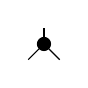
\begin{tikzpicture}[scale=0.2, black/.style={scale=0.5,draw,shape=circle,fill=black}]
	\node[black] (0) at (0, 0) {};
	\draw (1,-1) to (0);
	\draw (-1,-1) to (0);
	\draw (0) to (0,1);
	\end{tikzpicture}
}
\newcommand{\unit}{
	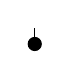
\begin{tikzpicture}[scale=0.2, black/.style={scale=0.5,draw,shape=circle,fill=black}]
	\node[black] (0) at (0, 0) {};
	\draw (0) to (0,1);
	\end{tikzpicture}
}
\newcommand{\comult}{
	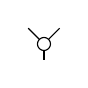
\begin{tikzpicture}[scale=0.2, black/.style={scale=0.5,draw,shape=circle,fill=white}]
	\node[black] (0) at (0, 0) {};
	\draw (1,1) to (0);
	\draw (-1,1) to (0);
	\draw (0) to (0,-1);
	\end{tikzpicture}
}

\newcommand{\counit}{
	\begin{tikzpicture}[scale=0.2, black/.style={scale=0.5,draw,shape=circle,fill=white}]
	\node[black] (0) at (0, 0) {};
	\draw (0) to (0,-1);
	\end{tikzpicture}
}

\newcommand{\antipode}{
	\begin{tikzpicture}[scale=0.2, black/.style={scale=0.5,draw,regular polygon,
		regular polygon sides=4,fill=white}]
	\node[scale=0.5, black] (0) at (0, 0) {$S$};
	\draw (0) to (0,-1);
	\draw (0) to (0,1);
	\end{tikzpicture}
}


\newcommand{\associativity}{
\begin{equation}
\begin{gathered}
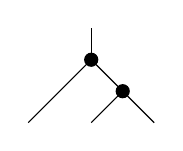
\begin{tikzpicture}[scale=0.8]
\node[scale=0.5,draw,circle,fill=black] (0) at (0,0.5) {};
\node[scale=0.5,draw,circle,fill=black] (1) at (0.5,0) {};
\draw (0) to (1);
\draw (-1,-0.5) to (0);
\draw (0,-0.5) to (1);
\draw (1,-0.5) to (1);
\draw (0) to (0,1);
\end{tikzpicture}
\end{gathered}
\, = \,
\begin{gathered}
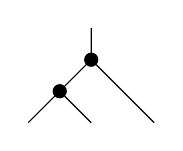
\begin{tikzpicture}[scale=0.8]
\node[scale=0.5,draw,circle,fill=black] (0) at (0.5,0.5) {};
\node[scale=0.5,draw,circle,fill=black] (1) at (0,0) {};
\draw (0) to (1);
\draw (-0.5,-0.5) to (1);
\draw (0.5,-0.5) to (1);
\draw (1.5,-0.5) to (0);
\draw (0) to (0.5,1);
\end{tikzpicture}
\end{gathered}
\end{equation}
}
\newcommand{\unitlaw}{
\begin{equation}
\begin{gathered}
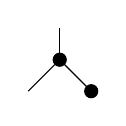
\begin{tikzpicture}[scale=0.8]
\node[scale=0.5,draw,circle,fill=black] (0) at (0,0.5) {};
\node[scale=0.5,draw,circle,fill=black] (1) at (0.5,0) {};
\draw (0) to (1);
\draw (-0.5,0) to (0);
\draw (0) to (0,1);
\end{tikzpicture}
\end{gathered}
\, = \,
\begin{gathered}
\begin{tikzpicture}[scale=0.8]
\draw (0,0) to (0,1);
\end{tikzpicture}
\end{gathered}
\, = \,
\begin{gathered}
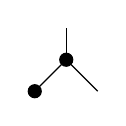
\begin{tikzpicture}[scale=0.8]
\node[scale=0.5,draw,circle,fill=black] (0) at (0,0.5) {};
\node[scale=0.5,draw,circle,fill=black] (1) at (-0.5,0) {};
\draw (0) to (1);
\draw (0.5,0) to (0);
\draw (0) to (0,1);
\end{tikzpicture}
\end{gathered}
\end{equation}
}
\newcommand{\coassociativity}{
\begin{equation}
\begin{gathered}
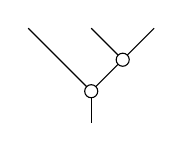
\begin{tikzpicture}[scale=0.8]
\node[scale=0.5,draw,circle,fill=white] (0) at (0,-0.5) {};
\node[scale=0.5,draw,circle,fill=white] (1) at (0.5,0) {};
\draw (0) to (1);
\draw (-1,0.5) to (0);
\draw (0,0.5) to (1);
\draw (1,0.5) to (1);
\draw (0) to (0,-1);
\end{tikzpicture}
\end{gathered}
\, = \,
\begin{gathered}
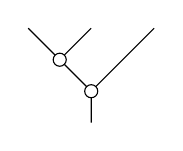
\begin{tikzpicture}[scale=0.8]
\node[scale=0.5,draw,circle,fill=white] (0) at (0.5,-0.5) {};
\node[scale=0.5,draw,circle,fill=white] (1) at (0,0) {};
\draw (0) to (1);
\draw (-0.5,0.5) to (1);
\draw (0.5,0.5) to (1);
\draw (1.5,0.5) to (0);
\draw (0) to (0.5,-1);
\end{tikzpicture}
\end{gathered}
\end{equation}
}
\newcommand{\counitlaw}{
\begin{equation}
\begin{gathered}
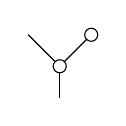
\begin{tikzpicture}[scale=0.8]
\node[scale=0.5,draw,circle,fill=white] (0) at (0,-0.5) {};
\node[scale=0.5,draw,circle,fill=white] (1) at (0.5,0) {};
\draw (0) to (1);
\draw (-0.5,0) to (0);
\draw (0) to (0,-1);
\end{tikzpicture}
\end{gathered}
\, = \,
\begin{gathered}
\begin{tikzpicture}[scale=0.8]
\draw (0,0) to (0,1);
\end{tikzpicture}
\end{gathered}
\, = \,
\begin{gathered}
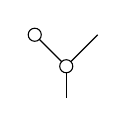
\begin{tikzpicture}[scale=0.8]
\node[scale=0.5,draw,circle,fill=white] (0) at (0,-0.5) {};
\node[scale=0.5,draw,circle,fill=white] (1) at (-0.5,0) {};
\draw (0) to (1);
\draw (0.5,0) to (0);
\draw (0) to (0,-1);
\end{tikzpicture}
\end{gathered}
\end{equation}
}

\newcommand{\bialgebralaw}{
\begin{equation}
\begin{gathered}
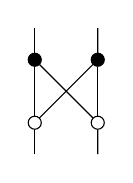
\begin{tikzpicture}[scale=0.8]
\node[scale=0.5,draw,circle,fill=white] (0) at (0,0) {};
\node[scale=0.5,draw,circle,fill=white] (1) at (1,0) {};
\node[scale=0.5,draw,circle,fill=black] (2) at (0,1) {};
\node[scale=0.5,draw,circle,fill=black] (3) at (1,1) {};
\draw (0) to (2);
\draw (0) to (3);
\draw (1) to (2);
\draw (1) to (3);
\draw (0,-0.5) to (0);
\draw (1,-0.5) to (1);
\draw (0,1.5) to (2);
\draw (1,1.5) to (3);
\end{tikzpicture}
\end{gathered}
\, = \,
\begin{gathered}
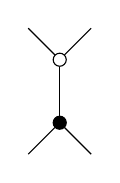
\begin{tikzpicture}[scale=0.8]
\node[scale=0.5,draw,circle,fill=black] (0) at (0.5,0) {};
\node[scale=0.5,draw,circle,fill=white] (1) at (0.5,1) {};
\draw (0) to (1);
\draw (0,-0.5) to (0);
\draw (1,-0.5) to (0);
\draw (0,1.5) to (1);
\draw (1,1.5) to (1);
\end{tikzpicture}
\end{gathered}
\end{equation}
}
\newcommand{\copylaw}{
\begin{equation}
\begin{gathered}
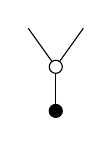
\begin{tikzpicture}[scale=0.7, squr/.style={scale=0.5,draw,regular polygon,
	regular polygon sides=4,fill=white}, black/.style={scale=0.5,draw,shape=circle,fill=black}, whit/.style={scale=0.5,draw,shape=circle,fill=white}]
\node[black] (0) at (0, 0) {};
\node[whit] (1) at  (0, 0.8) {};
\draw (0) to (1);
\draw (1) to (0.5,1.5);
\draw (1) to (-0.5,1.5);
\end{tikzpicture}
\end{gathered}
\, = \,
\begin{gathered}
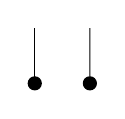
\begin{tikzpicture}[scale=0.7, black/.style={scale=0.5,draw,shape=circle,fill=black}]
\node[black] (0) at (0,0) {};
\node[black] (1) at (1,0) {};
\draw (0) to (0,1);
\draw (1) to (1,1);
\end{tikzpicture}
\end{gathered}
\end{equation}
}
\newcommand{\cocopylaw}{
	\begin{equation}
	\begin{gathered}
	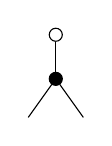
\begin{tikzpicture}[scale=0.7, squr/.style={scale=0.5,draw,regular polygon,
		regular polygon sides=4,fill=white}, black/.style={scale=0.5,draw,shape=circle,fill=black}, whit/.style={scale=0.5,draw,shape=circle,fill=white}]
	\node[whit] (0) at (0, 0) {};
	\node[black] (1) at  (0, -0.8) {};
	\draw (0) to (1);
	\draw (1) to (0.5,-1.5);
	\draw (1) to (-0.5,-1.5);
	\end{tikzpicture}
	\end{gathered}
	\, = \,
	\begin{gathered}
	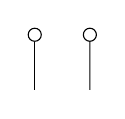
\begin{tikzpicture}[scale=0.7, black/.style={scale=0.5,draw,shape=circle,fill=white}]
	\node[black] (0) at (0,0) {};
	\node[black] (1) at (1,0) {};
	\draw (0) to (0,-1);
	\draw (1) to (1,-1);
	\end{tikzpicture}
	\end{gathered}
	\end{equation}
}
\newcommand{\hopflaw}{
	\begin{equation}
	\begin{gathered}
	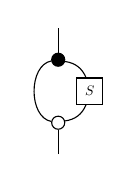
\begin{tikzpicture}[scale=0.8, squr/.style={scale=0.5,draw,regular polygon,
		regular polygon sides=4,fill=white}]
	\node[scale=0.5,draw,circle,fill=white] (0) at (0,0) {};
	\node[scale=0.5,draw,circle,fill=black] (1) at (0,1) {};
	\node[squr] (2) at (0.5,0.5) {$S$};
	\draw[bend left=80] (0) to (1);
	\draw[bend right] (0) to (2);
	\draw[bend right] (2) to (1);
	\draw (0,-0.5) to (0);
	\draw (0,1.5) to (1);
	\end{tikzpicture}
	\end{gathered}
	\, = \,
	\begin{gathered}
	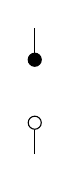
\begin{tikzpicture}[scale=0.8, squr/.style={draw,regular polygon,
		regular polygon sides=4,fill=white}]
	\node[scale=0.5,draw,circle,fill=white] (0) at (0,0) {};
	\node[scale=0.5,draw,circle,fill=black] (1) at (0,1) {};
	\draw (0,-0.5) to (0);
	\draw (0,1.5) to (1);
	\end{tikzpicture}
	\end{gathered}
	\, = \,
	\begin{gathered}
	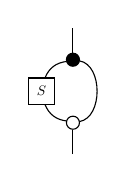
\begin{tikzpicture}[scale=0.8, squr/.style={scale=0.5,draw,regular polygon,
		regular polygon sides=4,fill=white}]
	\node[scale=0.5,draw,circle,fill=white] (0) at (0,0) {};
	\node[scale=0.5,draw,circle,fill=black] (1) at (0,1) {};
	\node[squr] (2) at (-0.5,0.5) {$S$};
	\draw[bend right=80] (0) to (1);
	\draw[bend left] (0) to (2);
	\draw[bend left] (2) to (1);
	\draw (0,-0.5) to (0);
	\draw (0,1.5) to (1);
	\end{tikzpicture}
	\end{gathered}
	\end{equation}
}
\newcommand{\modulelaw}{
	\begin{equation}
	\begin{gathered}
	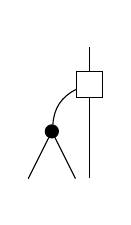
\begin{tikzpicture}[scale=0.6, squr/.style={draw,regular polygon,
		regular polygon sides=4,fill=white}, black/.style={scale=0.5,draw,shape=circle,fill=black}]
	\node (0) at (0, -2.2) {};
	\node[squr] (1) at (0, 0) {};
	\node (2) at (0, 1) {};
	\node[black] (3) at (-0.8, -1) {};
	\draw (0) to (1);
	\draw (1) to (2);
	\draw[bend left] (3) to (1);
	\draw (-1.3, -2) to (3);
	\draw (-0.3, -2) to (3);
	\end{tikzpicture}
	\end{gathered}
	\, = \,
	\begin{gathered}
	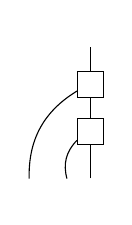
\begin{tikzpicture}[scale=0.6, squr/.style={draw,regular polygon,
		regular polygon sides=4,fill=white}, black/.style={draw,shape=circle,fill=black}]
	\node (0) at (0, -2.2) {};
	\node[squr] (1) at (0, 0) {};
	\node (2) at (0, 1) {};
	\node[squr] (3) at (0, -1) {};
	\draw (0) to (3);
	\draw (3) to (1);
	\draw (1) to (2);
	\draw (3) to (1);
	\draw[bend left] (-1.3, -2) to (1);
	\draw[bend left] (-0.5, -2) to (3);
	\end{tikzpicture}
	\end{gathered}
	\end{equation}
}
\newcommand{\comodulelaw}{
	\begin{equation}
	\begin{gathered}
	\begin{tikzpicture}[scale=0.6, squr/.style={draw,regular polygon,
		regular polygon sides=4,fill=white}, black/.style={scale=0.5,draw,shape=circle,fill=white}]
	\node (0) at (0, 2.2) {};
	\node[squr] (1) at (0, 0) {};
	\node (2) at (0, -2) {};
	\node[black] (3) at (-0.8, 1) {};
	\draw (0) to (1);
	\draw (1) to (2);
	\draw[bend right] (3) to (1);
	\draw (-1.3, 2) to (3);
	\draw (-0.3, 2) to (3);
	\end{tikzpicture}
	\end{gathered}
	\, = \,
	\begin{gathered}
	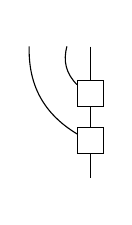
\begin{tikzpicture}[scale=0.6, squr/.style={draw,regular polygon,
		regular polygon sides=4,fill=white}, black/.style={draw,shape=circle,fill=black}]
	\node (0) at (0, 2.2) {};
	\node[squr] (1) at (0, 0) {};
	\node (2) at (0, -1) {};
	\node[squr] (3) at (0, 1) {};
	\draw (0) to (3);
	\draw (3) to (1);
	\draw (1) to (2);
	\draw (3) to (1);
	\draw[bend right] (-1.3, 2) to (1);
	\draw[bend right] (-0.5, 2) to (3);
	\end{tikzpicture}
	\end{gathered}
	\end{equation}
}
\newcommand{\intertwinerlaw}{
\begin{equation}
\begin{gathered}
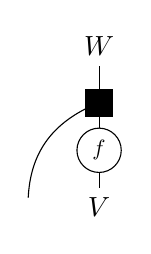
\begin{tikzpicture}[scale=0.6, squr/.style={draw,regular polygon,
	regular polygon sides=4,fill=black}]
\node (0) at (0, -2.2) {$V$};
\node[squr] (1) at (0, 0) {};
\node (2) at (0, 1.2) {$W$};
\node[scale=0.8,draw,circle] (3) at (0, -1) {$f$};
\draw (0) to (3);
\draw (3) to (1);
\draw (1) to (2);
\draw (3) to (1);
\draw[bend left] (-1.5, -2) to (1);
\end{tikzpicture}	
\end{gathered}
\, = \,
\begin{gathered}
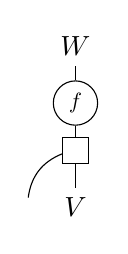
\begin{tikzpicture}[scale=0.6, squr/.style={draw,regular polygon,
	regular polygon sides=4,fill=white}]
\node (0) at (0, -2.2) {$V$};
\node[scale=0.8,draw,circle] (1) at (0, 0) {$f$};
\node (2) at (0, 1.2) {$W$};
\node[squr] (3) at (0, -1) {};
\draw (0) to (3);
\draw (3) to (1);
\draw (1) to (2);
\draw (3) to (1);
\draw[bend left] (-1, -2) to (3);
\end{tikzpicture}	
\end{gathered}
\end{equation}
}
\newcommand{\symAB}{
	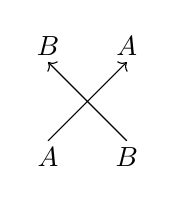
\begin{tikzpicture}[decoration={markings,mark=at position 0.5 with {\arrow{>}}}]
	\node (0) at (-0.5, -0.7) {$A$};
	\node (0) at (-0.5, 0.7) {$B$};
	\node (1) at (0.5, -0.7) {$B$};
	\node (1) at (0.5, 0.7) {$A$};
	\draw [->] (-0.5, -0.5) to (0.5, 0.5);
	\draw [->] (0.5, -0.5) to (-0.5, 0.5);
	\end{tikzpicture}
}

\newcommand{\symequation}{
	\begin{equation*}
	\begin{gathered}
	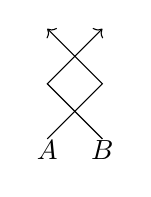
\begin{tikzpicture}[scale=0.7]
	\node (0) at (-1, -1.2) {$A$};
	\node (0) at (0, -1.2) {$B$};
	\draw [->] (-1, -1)--(0,0)--(-1,1);
	\draw [->] (0, -1)--(-1,0)--(0,1);
	\end{tikzpicture}
	\end{gathered}
	\, = \,
	\begin{gathered}
	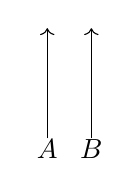
\begin{tikzpicture}[scale=0.7]
	\node (0) at (-0.8, -1.2) {$A$};
	\node (0) at (0, -1.2) {$B$};
	\draw [->] (-0.8, -1)--(-0.8,1);
	\draw [->] (0, -1)--(0,1);
	\end{tikzpicture}
	\end{gathered}
	\end{equation*}
}

\newcommand{\cupA}{	
	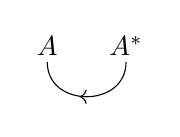
\begin{tikzpicture}[decoration={markings,mark=at position 0.5 with {\arrow{<}}}]
	\node (0) at (0, 0.2) {$A$};
	\node (1) at (1, 0.2) {$A^*$};
	\draw [bend right=90, looseness=1.5, postaction=decorate] (0,0) to (1,0);
	\end{tikzpicture}}

\newcommand{\capA}{	
	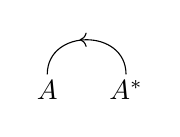
\begin{tikzpicture}[decoration={markings,mark=at position 0.5 with {\arrow{<}}}]
	\node (0) at (0, -0.2) {$A$};
	\node (1) at (1, -0.2) {$A^*$};
	\draw [bend left=90, looseness=1.5, postaction=decorate] (0,0) to (1,0);
	\end{tikzpicture}}

\newcommand{\snake}{
	\begin{equation*}
	\begin{gathered}
	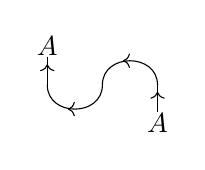
\begin{tikzpicture}[scale=0.7,decoration={markings,mark=at position 0.5 with {\arrow{<}}}]
	\node (0) at (0, 0.7) {$A$};
	\node (4) at (2, -0.7){$A$};
	\draw [bend right=90, looseness=1.5, postaction=decorate] (0, 0) to (1, 0);
	\draw [bend left=90, looseness=1.5, postaction=decorate] (1, 0) to (2, 0);
	\draw [postaction=decorate] (2, 0) to (2, -0.5);
	\draw [postaction=decorate] (0, 0.5) to (0, 0);
	\end{tikzpicture}
	\end{gathered}
	\, = \,
	\begin{gathered}
	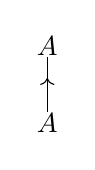
\begin{tikzpicture}[scale=0.7,decoration={markings,mark=at position 0.5 with {\arrow{<}}}]
	\node (0) at (0, 0.7) {$A$};
	\node (4) at (0, -0.7){$A$};
	\draw [postaction=decorate] (0, 0.5) to (0, -0.5);
	\end{tikzpicture}
	\end{gathered}
	\end{equation*}}

\newcommand{\snakestar}{
	\begin{equation*}
	\begin{gathered}
	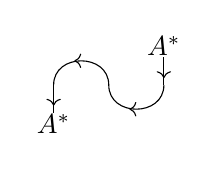
\begin{tikzpicture}[scale=0.7,decoration={markings,mark=at position 0.5 with {\arrow{<}}}]
	\node (0) at (0, -0.7) {$A^*$};
	\node (4) at (2, 0.7){$A^*$};
	\draw [bend left=90, looseness=1.5, postaction=decorate] (0, 0) to (1, 0);
	\draw [bend right=90, looseness=1.5, postaction=decorate] (1, 0) to (2, 0);
	\draw [postaction=decorate] (2, 0) to (2, 0.5);
	\draw [postaction=decorate] (0, -0.5) to (0, 0);
	\end{tikzpicture}
	\end{gathered}
	\, = \,
	\begin{gathered}
	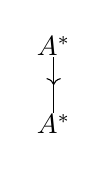
\begin{tikzpicture}[scale=0.7,decoration={markings,mark=at position 0.5 with {\arrow{>}}}]
	\node (0) at (0, 0.7) {$A^*$};
	\node (4) at (0, -0.7){$A^*$};
	\draw [postaction=decorate] (0, 0.5) to (0, -0.5);
	\end{tikzpicture}
	\end{gathered}
	\end{equation*}
}

\newcommand{\fusionijk}{
	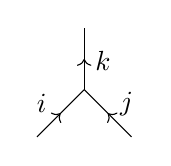
\begin{tikzpicture}[scale=0.6,decoration={markings,mark=at position 0.5 with {\arrow{>}}}]
	\node (0) at (-0.9, -0.3) {$i$};
	\node (1) at (0.9, -0.3) {$j$};
	\node (2) at (0.4, 0.6) {$k$};
	\draw [postaction=decorate] (-1, -1) to(0,0);
	\draw [postaction=decorate] (1,-1) to (0,0);
	\draw [postaction=decorate] (0,0) to (0,1.3);
	\end{tikzpicture}}
%%%%%%%%%%%%%%%%%%%%%%%%%%%%%%%%%%%%%%%%%%%%%%%%%%%%%%%%%%%%%%%%%%%%%%%%%%%%%%%%%%%%%%%%%%%%%%%%%%%%%%%%%%%%%%%%%%%%%%%%%%%%%%%%%%%%%%%%%%%%%%%%%%%%%%%%%%%%%%%%%%%%%%%%%%%%%%%%%%%%


\begin{document}

\section{Quantum Computation}

\subsection{Topological Quantum Computation}

\subsubsection{From categories to computation}
In the previous section we saw that categories can be interpreted as physical process theories. In a very similar way, we can interpret objets as data types and morphisms as computational processes, so that any category corresponds to a theory of computation. Monoidal categories are ones where parallel computation is possible. Quantum computation is a model in which data is encoded in the state of quantum systems (particles) and processes are quantum transformations of the system. A computation consists of the preparation of some quantum states, their manipulation and measurement. This procedure is repeated in order to collect statistics and approximate density distributions. The unit of information in quantum computation is called qubit by analogy with the classical bit. A qubit is a two-level quantum system, that is a Hilbert space of dimension $2$ which is denote by $\mathbb{C}^2$\\
Modular categories are models for topological quantum computation (TQC) in the sense of \cite{Kitaev03} or \cite{Rowell17}. TQC has been studied extensively in recent years as it allows for fault-tolerant quantum computation. In this model data is encoded in non-abelian anyons and quantum gates are obtained by braiding those particles. Topologically equivalent braids implement the same quantum process so that small perturbations of particle world-lines do not affect the computation and gates are topologically protected from decoherence.
Another reason for studying topological quantum computation is that some TQC models allow to approximate the Jones polynomial in polynomial time, a problem that is believed to be untractable classically (it is in the complexity class $\# P$) .\\
The problem of building a topological quantum computer has been addressed by various authors \cite{Kitaev03} [cite freedman]. The difficulty arises in the two-dimensional nature of anyons. Indeed those are only known to arise as quasi-particle excitations on two-dimensional fluids at low temperature, an experimentally difficult setup which was never achieved for non-abelian excitations.\\
A topological quantum computer runs as follows \cite{Rowell17}:
\begin{definition}[TQC]
	\begin{enumerate}
		\item Creation of anyon pairs from the vacuum to encode the information as a quantum state.
		\item Braiding those anyons performs a quantum gate on the state.
		\item fusing neighbouring anyons and observing the resulting anyon type corresponds to a projective measurement on the system.
	\end{enumerate}
\end{definition}
The computation result is the approximation to a probability distribution (over measurement outcomes) obtained by repeating the procedure polynomially many times and recording the output anyon types. Note that if we postselct on the vacuum sector to be the output anyon type we are effetively approximating an invariant of links. Indeed any process in TQC starting and ending in the vacuum sector is a link, formed by the particle trajectories in space-time (i.e the briading process). The time evolution of the system $V$ must be a unitary operator, so that any braiding process on $n$ particles induces the evaluation of some representation $\beta \rightarrow U_\beta$ of the braid group $B_n$.\\
In order to make sure the braiding process is a unitary transformation of the state space we will impose one further constraint on our categorical model of computation: unitarity of the braids in the modular category in question.\\
Take the fusion space to be our computational hilbert space.\\
Topological qudits are usually encoded as fusion tree basis elements\\
Topologial gates: braids (can express as action of the braid group) + measurements (=fusions and associators).

\subsubsection{Fibonacci anyons}
We now look back at example [ref] on Fibonacci anyons and show how to compute in the model.
Recall we have only two particle types: the vacuum sector $1$ and the non-trivial $\tau$ such that:
$$\tau \otimes \tau = 1 \oplus \tau$$
$\tau$ and $1$ are their own anti-particles so we don't need to distinguish particles and antiparticles by wrinting arrows on wires.
We can write the basis of the two dimensional space $\tau \otimes \tau$ as:
\begin{center}
	\begin{tikzpicture}
		\node (0) at (0.3, 0.3) {$\tau$};
		\node (0) at (-0.7, -0.3) {$\tau$};
		\node (0) at (0.7, -0.3) {$\tau$};
		\draw (-0.5, -0.5)--(0,0)--(0,0.5);
		\draw (0.5, -0.5)--(0,0);
	\end{tikzpicture}
	\quad
	\begin{tikzpicture}
	\node (0) at (0.3, 0.3) {$1$};
	\node (0) at (-0.7, -0.3) {$\tau$};
	\node (0) at (0.7, -0.3) {$\tau$};
	\draw (-0.5, -0.5)--(0,0)--(0,0.5);
	\draw (0.5, -0.5)--(0,0);
	\end{tikzpicture}
\end{center}
The fusion space $V_{\tau^{\otimes 3}}^\tau$ is two dimensional, we will take it as our computational space and write the computational basis as:
\begin{center}
	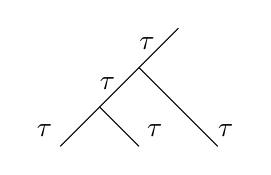
\begin{tikzpicture}
	\node (0) at (0.1, 0.3) {$\tau$};
	\node (0) at (-0.7, -0.3) {$\tau$};
	\node (0) at (0.7, -0.3) {$\tau$};
	\node (0) at (0.6, 0.8) {$\tau$};
	\node (0) at (1.6, -0.3) {$\tau$};
	\draw (-0.5, -0.5)--(0,0)--(0.5,0.5)--(1,1);
	\draw (0.5, -0.5)--(0,0);
	\draw (1.5, -0.5)--(0.5,0.5);
	\end{tikzpicture}
	\quad
	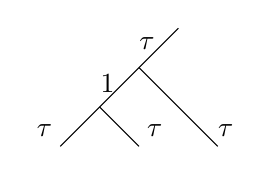
\begin{tikzpicture}
	\node (0) at (0.1, 0.3) {$1$};
	\node (0) at (-0.7, -0.3) {$\tau$};
	\node (0) at (0.7, -0.3) {$\tau$};
	\node (0) at (0.6, 0.8) {$\tau$};
	\node (0) at (1.6, -0.3) {$\tau$};
	\draw (-0.5, -0.5)--(0,0)--(0.5,0.5)--(1,1);
	\draw (0.5, -0.5)--(0,0);
	\draw (1.5, -0.5)--(0.5,0.5);
	\end{tikzpicture}
\end{center}
Let's denote by $\ket{0}, \ket{1}$ these basis states. Another basis is given by fusing the left-most two anyons first:
\begin{center}
	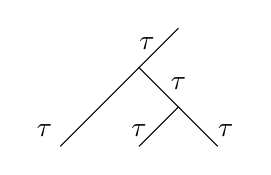
\begin{tikzpicture}
	\node (0) at (1, 0.3) {$\tau$};
	\node (0) at (-0.7, -0.3) {$\tau$};
	\node (0) at (0.5, -0.3) {$\tau$};
	\node (0) at (0.6, 0.8) {$\tau$};
	\node (0) at (1.6, -0.3) {$\tau$};
	\draw (-0.5, -0.5)--(0,0)--(0.5,0.5)--(1,1);
	\draw (0.5, -0.5)--(1,0);
	\draw (1.5, -0.5)--(0.5,0.5);
	\end{tikzpicture}
	\quad
	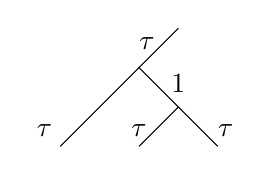
\begin{tikzpicture}
	\node (0) at (1, 0.3) {$1$};
	\node (0) at (-0.7, -0.3) {$\tau$};
	\node (0) at (0.5, -0.3) {$\tau$};
	\node (0) at (0.6, 0.8) {$\tau$};
	\node (0) at (1.6, -0.3) {$\tau$};
	\draw (-0.5, -0.5)--(0,0)--(0.5,0.5)--(1,1);
	\draw (0.5, -0.5)--(1,0);
	\draw (1.5, -0.5)--(0.5,0.5);
	\end{tikzpicture}
\end{center}
And we denote them by $\ket{+}, \ket{-}$. These two bases are linked by a unitary $2 \times 2$ transformation $F:= F^\tau_{\tau^{\otimes 3}}$ given by the solution of the following system:
$$ \ket{0} = F_{0+} \ket{+} + F_{0-} \ket{-}$$
$$ \ket{1} = F_{1+} \ket{+} + F_{1-} \ket{-}$$
To derive the form of the $F$-matrix we need to consider the pentagon axiom. It turns out that for the Fibonacci model the pentagon is enough to derive the $F$-matrix but it is not the case in general. The resulting $F$-matrix is \cite{Simon16}:
\begin{center}
	$\begin{bmatrix}
	\phi^{-1} & \phi^{-\frac{1}{2}} \\
	\phi^{-\frac{1}{2}} & -\phi^{-1}
	\end{bmatrix}$
\end{center}
where $\phi = \frac{\sqrt{5}-1}{2}$.

\subsubsection{Kitaev's quantum double model}
Fix a group $G$, and suppose we have particles living in state space $\mathbb{C}G$ (the group agebra). We will build a special case of Kitaev's quantum double model \cite{Kitaev03}, in order to see directly the connection with the category $Rep(DG)$.\\
First of all let us consider 4 types of linear operators on $\mathbb{C}G$: $L^g_\pm$, $T^h_\pm$ (using the notation from \cite{Kitaev03}). Indexed by elements $g,h \in G$, and defined as follows:
\begin{equation}
	\begin{aligned}
	L^g_+ \ket{z} = \ket{gz} \quad& L^g_- \ket{z} = \ket{zg^{-1}}\\
	T^h_+ \ket{z} = \delta_{h,z} \ket{z} \quad& T^h_- \ket{z} = \delta_{h^{-1},z} \ket{z}
	\end{aligned}	 
\end{equation}
Now, consider the trivial lattice on a torus with particles on the edges, i.e a square with opposite edges identified as follows:
\begin{center}
	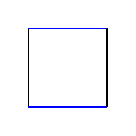
\begin{tikzpicture}[decoration={markings,mark=at position 0.5 with {\arrow{>}}}]
		\draw (0,0)--(0,1);
		\draw (1,0)--(1,1);
		\draw[blue] (0,1)--(1,1);
		\draw[blue] (0,0)--(1,0);
	\end{tikzpicture}
\end{center}
For the moment take this lattice as our system, note that states are generated by pairs of elements of $G$, each labelling one edge of the lattice. Let's say that $L^g_\pm(0)$, $L^g_\pm(1)$ and $T^h_\pm(0)$ $T^h_\pm(1)$ are $L_\pm$ and $T_\pm$ operators acting on the first and second particle. Note that in this configuration, we have only one plaquette and one vertex, we will only need to define two types of operators on the lattice, indexed by elements of $G$. For $g,h \in G$ define:
\begin{equation}
	\begin{aligned}
	A_g &= L^g_+(0) L^g_+(1) L^g_-(0) L^g_-(1)\\
	P_h &= \sum_{h_1h_2h_3h_4=h} T^{h_1}_+(0) T^{h_2}_+(1) T^{h_3}_-(0) T^{h_4}_-(1)
	\end{aligned}
\end{equation}
From a physical point of view $P_h$ operators can be understood as measuring the magnetic flux of the system and $A_g$ are symmetry transformations on the charge. Flux measurements are projection $P_h \in \mathbb{C}G^*$ onto flux sector $h$. The allowed residual global symmetry transformations are then implemented via $A_g$ for $g \in N(h)$. \\
Naturally the projectors form a Von Neumann family and satisfy 
$$P_hP_{h'}= \delta_{h,h'} P_h.$$ 
Operators $A_g$ are global symmetry transformation 
$$A_gA_h = A_gh$$
and affect the fluxes via conjugation:
\begin{equation}\label{doublemult}
A_gP_h = P_{ghg^{-1}}A_g
\end{equation}
(this was shown was shown by Kitaev \cite{Kitaev03}). Operators $A_g$ and $P_h$ generate the algebra $DG$. So the quantum double construction allows to capture both global symmetry transformations and projective measurements in one algebraic structure. It is easy to check, rewriting the definition, that the following is true. 
\begin{proposition}
	For any finite group $G$, its quantum double $D(G)$ is the algebra generated by $\{P_hA_g\}_{h,g\in G}$ with multiplication induced by (\ref{doublemult}) comultiplication and antipode as defined in [first section]. 
\end{proposition}
$D(G)$ has a natural quasi-triangular structure witnessed by the universal R-matrix $R=\sum_{g,h \in G}P_he \otimes P_hg$, making $RepDG$ braided.\\
Kitaev then builds a Hamiltonian for the system and shows that the sectors of this Hamiltonian are precisely the irreducible representations of $DG$. Here we will skip this part of the reasoning and rely on the intuition that the operators $A_g$ and $P_h$ correspond to the symmetries of the system, i.e the dynamics which are `constantly being applied'. So the allowed processes of the systems are processes that commute with all of those operators, i.e the system lives in a representation of $DG$ and the allowed processes are intertwiners. We obtain the process theory $Rep(DG)$. Note that because we chose our lattice to be trivial, in the model as we described it the overall dimension of the system is at most $|G|^2$ and we cannot obtain higher dimensional representations. This issue was directly avoided by Kitaev in his presentation \cite{Kitaev03}, by allowing the lattice to be arbitrairy (embedded in some manifold) and defining $A_g$ and $P_h$ operators on sites (i.e vertices together with a plaquette). For each site $a=(s,p)$ where $s$ is a vertex and $p$ a plaquette, we have operators $A_g(a)$ and $P_h(a)$ which generate the quantum double algebra. An excitation is then a state of some non-trivial irreducible representation of $DG$ being created at some site $a$ on the lattice. Those excitations have anyonic behaviour. In what follows we will assume the lattice was `layered' enough so that we can create more than one excitation and we can move around without fusing them. If the lattice is big enough we have obtained a practical implementation of anyons whose behaviour is described by the modular category $Rep(DG)$. When $G$ is abelian, we only have abelian anyons which are very unlikely to be universal for quantum computation. It was shown by Kitaev that if $G=S_5$ the model is universal for quantum computation. In [cite Lahtinen] the $G=S_3$ model was considered but not shown to be universal.\\  
In order to understand the possible anyon types in the model induced by finite group $G$, we must study the irreducible representations of the quantum double finite group algebra $DG$. This has been done by Gould \cite{Gould93}, who showed that irreducible representations of $DG$ are obtained in the following way.\\
Let $\{C_i\}_{i=1}^n$ be the distinct conjugacy classes in $G$. To each of those conjugacy classes corresponds a centralizer subgroup $N_i$ (two choices of representatives for $C_i$ yield isomorphic centralizer subgroups). Then for any irreducible representation $(\alpha,V^i_\alpha)$ of $N_i$ with basis elements $v^\alpha_j$, let $V_{i,\alpha} = \mathbb{C}C_i \otimes V^i_\alpha$, this has basis $\{ \ket{k,v^\alpha_j} \}_{j=1,...,dim\alpha}^{k\in C_i}$ and forms an irreducible representation of $D(G)$ under the action 
\begin{equation}
P_hg\ket{k,v^\alpha_j} = \delta_{h,gkg^{-1}} \ket{h,\alpha(h^{-1}gk)v^\alpha_j}
\end{equation}
and the $\{V_{i,\alpha}\}$ is the complete set of irreducible representations.

\begin{example}[Kitaev's Toric code]
	The case where $G \simeq \mathbb{Z}_2$ gives rise to Kitaev's toric code. Note that $D(\mathbb{Z}_2) \simeq \mathbb{C}(\mathbb{Z}_2\times \mathbb{Z}_2^\star)$, so that there are $4$ irreducible representations, all of which are 1-dimensional. Each of those corresponds to a different type of excitation.  Let $x$ and $y$ be the generators of the group. The trivial representation is the trivial excitation (or `no excitation'). The other irreducible representations are obtained by mapping $x$ and $y$ to order $2$  elements of $\mathbb{C}$. We obtain two bosons, when both get sent to $-1$ or $i$ and one fermions when $x \mapsto -1$ and $y \mapsto i$. 
\end{example}

\subsection{Permutational Quantum Computing}
This section is about a model of quantum computation introduced by Jordan \cite{Jordan09}. We will first introduce the model as it appears in \cite{Jordan09} and then give a categorical presentation not present in the literature which will allow us to generalize the model and compare it to other computational models.

\subsubsection{Jordan's model}
Let $\mathcal{L}$ be an $n$-qubit quantum system. Basis states of an $n$-qubit quantum systems are often specified by listing eigenvalues of Pauli-$Z$ operators applied to each qubit, which is known as computational basis.
Permutational quantum computing (PQC) works with another choice of basis states: eigenstates of complete set of commuting spin measurements on qubit subsets. Let us fix a finite set $I=\{1,2,3...,n\}$ indexing the qubits. With a convention that $\hbar = 1$, the spin of the $k$-th qubit is defined by a triple:
\begin{align*}
\vec{S}_k &= \frac{1}{2} \left( X_k, \, Y_k, \,Z_k \right),
\end{align*}
where $X_k$, $Y_k$ and $Z_k$ denote the Pauli $X$,$Y$ and $Z$ operators on the $k$-th qubit. The total spin operator of a qubit subset $A$  is given by:
\begin{align*}
S_A^2 &= \left( \sum_{k \in A} \vec{S}_k \right) \cdot  \left( \sum_{k \in A} \vec{S}_k \right)\,,
\end{align*} 
and we will use $S^2$ to denote the spin operator on the set of all qubits. 
Let 
$$Z_A = \frac{1}{2} \sum_{k \in A} Z_k $$ 
denote the total $Z$-spin operator on qubit subset $A$ and we label by $Z$ the total $Z$-operator applied to all qubits (i.e $Z=Z_I$). $Z$ and $S^2$ commute and stabilize an eigenspaces labeled by quantum numbers $J$ and $M$: 
\begin{equation}
S^2  \ket{J, \, M} = J (J +1 ) \ket{J, \, M},  \\
Z \ket{J, \, M} = M \ket{J, \, M},
\end{equation} 
where $J$ is the total spin of all qubits and $M$ takes values $ -J \leq M \leq J$ in an integer steps. There are therefore $2J + 1$ $Z$-operator eigenstates for each $J$ and we will refer to this degeneracy as $M$-degeneracy. \\
Now, it is easy to see that the operators $S_A^2$ and $S_B^2$ on sets $A, B$ commute if and only if $A$ and $B$ are disjoint or one is subset of the other. We can therefore give a complete set of commuting operators on $I$:
\begin{equation} \label{comS}
S_{\lbrace12\rbrace}^2, \, S_{\lbrace123\rbrace}^2, \, \ldots S^2, \, Z
\end{equation}
In practice, this means that if we have $n$ qubits, measuring each of those operators yields a a sequence of outcomes $j_{12}, j_{123}, ... , J, M$ (the eigenvalues of each operator) which tests for some state of $\mathcal{J}$. Dually, allowing superselection on the outcomes of each measurement we have also defined a preparation recipe. This choice of basis states is known as \textit{sequential coupling}.\\
The $j$-quantum numbers on sets of qubits $A,B$ combine according to the angular addition rules \cite{Woit17}: 
\begin{align*}
|j_A - j_B| \leq j_{A \cup B} &\leq j_A + j_B, \\
j_{A \cup B} + j_A + j_B & \in \mathbb{Z},
\end{align*}
For example if $n=3$, there are two ways to obtain $J=\frac{1}{2}$ eigenstate of three spins - either by adding a qubit to a two-qubit singlet $(J=0)$ state, or by adding a qubit to a triplet $(J=1)$ \cite{Pauncz67}.
We can picture those states as labeled binary trees with $n$ leaves, which we refer to as labeled recoupling diagrams. For instance, for $n=3$ we have:

Note that the shape of those binary trees is induced by the choices (\ref{comS}). Every rooted binary tree shape with $n$ leaves (which we will refer to as recoupling diagram) yields a different choice of complete set of commuting observables, and therefore a different choice of basis for $\mathcal{L}$. And clearly there are $2^n$ of labelled recoupling diagrams for every recoupling diagram, one for each basis state.
A computation in PQC is given by the following procedure:
\begin{definition}[PQC]\label{pqcomputation} 
	Given a permutation $\pi$: %and an error threshold $\epsilon$:
	\begin{enumerate}
		\item Prepare a simultaneous eigenstate $\ket{\lambda} = \ket{j_{12}, j_{123}, \ldots, J, M}$ of $ S_{12}^2, \, S_{123}^2, \, \ldots S^2, Z$. Such basis (ie. the sequentially coupled basis) plays the role of computational basis .  %Once the fusion diagram is fixed, this can be a superposition over different tree labelings. 
		%The state can be in principle preprocessed by polarizing the spins by external magnetic field {\color{blue} [Improve the state preparation argument]}.
		\item Measure the following  set of observables: $S_{ \pi(1)\pi(2) }^2, \, S_{ \pi(1)\pi(2)\pi(3) }^2, \, \ldots S^2, Z$. This is equivalent to applying a sequence of \textsf{SWAP} gates $U_\pi$ in the quantum circuit model and measuring a $J$-spin eigenstate $\ket{x} = \ket{j_{12}', j_{123}', \ldots, J', M'}$ in the sequentially coupled basis.	
		\item The computing result is obtained by repeating steps 1 and 2 polynomially many times to yield an approximation of the probability distribution $P_\pi (x|\lambda) = | \bra{x} U_\pi \ket{\lambda}|^2 $.
	\end{enumerate}
\end{definition}
In his paper \cite{Jordan09}, Jordan shows that PQC can approximate the irreducible representations of the symmetric group in polynomial tyme. This is a relatively surprising result as this problem no classical polynomial time algorithm is known that solves the same problem. This hints that although the the PQC model seems trivial in comparison with other quantum computation models it is still superior to classical computation. Any PQC computation (\ref{pqcomputation}), corresponds to a sequence of phase and racah moves.
\begin{definition}[Phase and Racah moves]
\end{definition}
\begin{theorem}[Biedenharn-Louck \cite{Aquilanti09}] 
	Let $A,B,C$ be disjoint sets of qubits and use the shorthand $AB := A \cup B$.
	Any quantum state corresponding to a labelled recoupling diagram can be transformed to a superposition of sequentially coupled labelled recoupling diagram states using a $poly(n)$ sequence of Racah and Phase moves.
\end{theorem}
Those moves have a general categorical description as we will see.

\subsubsection{Categorical PQC}
The theory of permutational quantum computing is based on the following abstract ingredients:
\begin{enumerate}
	\item A tensor product to model many-body quantum systems
	\item A direct product to model superpositions of particle types.
	\item A set of labels of particle types (with antiparticle for each type) generating all other systems together with fusion rules which account for coupling of those particle types.
	\item A permutational structure, i.e the possibility to permute particle positions, i.e phase moves
	\item The Racah or $F$ moves which models changes of basis.
	\item Underlying Hilbert spaces which account for the quantum mechanical nature of the model.
\end{enumerate}
Let us build a class of categories which account for all those ingredients. As already argued in the previous section we need the structure of a tensor category in order to model many-body quantum systems together with superpositions. We then require the category to contain a simple object for each particle type and to be semisimple so that we obtain fusion rules (see appendix). Note that we do not require there to be finitely many simple objects as in the anyonic case. Indeed note that if we want a theory to reproduce Jordan's model for any chosen number of particles ($n$), the theory must contain infinitely many particle types, one for each half-integer value (value of angular momentum). We must also require the category to be rigid so that for we have antiparticles for each particle type. A tensor category is monoidal so it comes with associators which precisely model the equivalent of the Racah moves. For the permutational structure we require the theory to have a symmetric structure. And finally, if we want to recover finite dimensional Hilbert spaces underlying the objects of our theory we can impose the existence of a forgetful functor to $FHilb \simeq FVect$. Putting it all together we have obtained a rigid semisimple symmetric tensor category $\cat$ equipped with a fiber functor $F: \cat \rightarrow FVect$. We will call those categories Tannakian for our purposes.\\
The following theorem shows that any group and supergroup induces a model for permutational quantum computation.
\begin{theorem}[Doplicher-Roberts]
	If $\mathcal{C}$ is a rigid semisimple symmetric tensor category equipped with a fiber functor to $Vect$ then $\mathcal{C}$ is symmetrically monoidally equivalent to $Rep(G)$ for $G$ some group (if the twist is trivial) or some supergroup (if the twist is -1).
\end{theorem}
And in fact we recognize Jordan's model as the theory of representations of the special unitary group.
\begin{proposition}
	Jordan's qubit model $\mathcal{J}_2$ is the category of representations of $SU(2)$.
\end{proposition}
\begin{proof}
	Irreducible representations of $SU(2)$ are precisely indexed by half-integer values and the fusion rules given by angular addition rules \cite{Woit17}.
\end{proof}
We can easily see that defining $\mathcal{J}_d := Rep(SU(d))$ we obtain the corresponding qu$d$it model for permutational quantum computation. The permutational structure of the categories under observation, is tightly linked to the symmetric group $S_n$. In his model, Jordan builds an algorithm to compute representations of $S_n$, this can be done in any PQC category.
\begin{proposition}
	Any Tannakian category $\cat$ induces representations of the symmetric group $S_n$ for any $n\in \mathbb{N}$.
\end{proposition}
\begin{proof}
	Fix $n \in \mathbb{N}$ and a simple object $a \in obj(\cat)$ then $S_n$ acts on $a^{\otimes n}$ by permutations, and this clearly defines a module as we can consider $a$ as a vector space using the fiber functor.
\end{proof}


\begin{example}[Permutational quantum computation in $Rep(S_3)$]
\end{example}

\begin{example}[Approximation of Dijkgraaf-Witten link invariants]
	The link invariant essentially counts homomorphisms from the fundamental group
	of the link complement to the group G. (cite Zhenghan?)
\end{example}

%%%%%%%%%%%%%%%%%%%%%%%%%%%%%%%%%%%%%%%%%%%%%%%%%%%%%%%%%%%%%%%%%%%%%%%%%%%%%%%%%%%%%%%%%%%%%%%%%%%%%%%%%%%%%%%%%%%%%%%%%%%%%%%%%%%%%%%%%%%%%%%%
%%%%%%%%%%%%%%%%%%%%%%%%%%%%%%%%%%%%%%%%%%%%%%%%%%%%%%%%%%%%%%%%%%%%%%%%%%%%%%%%%%%%%%%%%%%%%%%%%%%%%%%%%%%%%%%%%%%%%%%%%%%%%%%%%%%%%%%%%%%%%%%%
\subsection{A braided representation of quantum computation}
For an abelian group $G$, we have seen that $Rep(DG)$ doesn't contain enough states to model preparations and measurements. But we will see that for suitably chosen $G$, $Rep(DG)$ contains a universal set of gates as braids. In this section we use functorial boxes \cite{Mellies06} to map the braided pictures in $Rep(DG)$ down to $Hilb$ and obtain a braided representation of quantum gates. This will allow us to to describe preparations and measurements in $Hilb$ and quantum gates as boxed braids from $Rep(DG)$.\\
We know from [drinfeld center section] that $Rep(DG) \simeq \mathcal{D}_G^{lr}$, so specifying an object of $Rep(DG)$ just corresponds to choosing a vector space $V$ with a left $G$-module structure  and right $G$-comodule structure.\\
Let $G:= \mathbb{Z}_2$, the reason why we chose this group will become apparent later on, many other choices are possible. Let us denote the standard basis of $\mathbb{C}G$ by $\{ \ket{0}, \ket{1}\}$. This has natural Hopf algebra structure with multiplication given by $\ket{i}\otimes \ket{j} \mapsto \ket{i+j}$ (where $+$ is addition modulo $2$) and comultiplication given by the copy map $\ket{i} \mapsto \ket{i}\otimes \ket{i} $.\\
We now choose a two-dimensional object of $Rep(DG)$ to serve as our qubit. Take $V=\mathbb{C}^2$ with the $Z$ $G$-action (i.e $Z$-phases) and $X$ $G$-coaction (i.e $X$ projective measurement).\\



\bibliographystyle{unsrt}
\bibliography{refs}

\end{document}
